%%%%%%%%%%%%%%%%%%%%%%%%%
%% Header for standard beamer presentation
%%
%%  PresentationHeader.tex
%%
%%%%%%%%%%%%%%%%%%%%%%%%%

\documentclass[english,10pt]{beamer}

%%%%%%%%%%%%%%%%%%%%
%% Include general header where common packages are defined
%%%%%%%%%%%%%%%%%%%%

% general packages without options
\usepackage{amsmath,amssymb,bbm}




%%%%%%%%%%%%%%%%%%%%
%% Idem general commands
%%%%%%%%%%%%%%%%%%%%

%%% Commands

\newcommand{\noun}[1]{\textsc{#1}}


%% Math

% Operators
\DeclareMathOperator{\Cov}{Cov}
\DeclareMathOperator{\Var}{Var}
\DeclareMathOperator{\E}{\mathbb{E}}
\DeclareMathOperator{\Proba}{\mathbb{P}}

\newcommand{\Covb}[2]{\ensuremath{\Cov\!\left[#1,#2\right]}}
\newcommand{\Eb}[1]{\ensuremath{\E\!\left[#1\right]}}
\newcommand{\Pb}[1]{\ensuremath{\Proba\!\left[#1\right]}}
\newcommand{\Varb}[1]{\ensuremath{\Var\!\left[#1\right]}}

% norm
\newcommand{\norm}[1]{\| #1 \|}


% amsthm environments
\newtheorem{definition}{Definition}



%% graphics

% renew graphics command for relative path providment only ?
%\renewcommand{\includegraphics[]{}}






\usetheme{Warsaw}

\setbeamertemplate{footline}[text line]{}
\setbeamercolor{structure}{fg=purple!50!blue, bg=purple!50!blue}

\setbeamercovered{transparent}


% shortened command for a justified frame
\newcommand{\jframe}[2]{\frame{\frametitle{#1}\justify{#2}}}



%%%%%%%%%%%%%%%%%%%%%
%% Begin doc
%%%%%%%%%%%%%%%%%%%%%

\begin{document}


\title{Towards Coupling Transportation Networks and City Growth in Complex Urban Systems Models
}


\author{J.~Raimbault$^{1,2}$}

\institute{$^{1}$G{\'e}ographie-Cit{\'e}s (UMR 8504 CNRS)\\
$^{2}$LVMT (UMR-T 8904 IFSTTAR)}


\date{Thesis Progress Meeting\\
March 10th 2015}


%%%%%%%%%%%%%%%%%%%%%%%%%%%%%%%%
\begin{frame}
\titlepage
\end{frame}

\begin{frame}
\tableofcontents
\end{frame}
%%%%%%%%%%%%%%%%%%%%%%%%%%%%%%%%



%%%%%%%%%%%%%%%%%%%%%%%%%%%%%%%%
\section{General Presentation}

\subsection{Context}


\begin{frame}
\frametitle{Scientific Context}
\vfill{}
\begin{justify}
Interactions between urban development and transportation network are considered to be central in dynamics of complex urban systems at any spatial and temporal scale~\cite{bretagnolle:tel-00459720}\cite{offner1993effets}. As many underlying time scales are involved in dynamics, very few modeling efforts have been done towards models simulating simultaneously both growths.\\
\vfill{}
Such geographical models would have both
\begin{itemize}
\item theoretical interest, in understanding processes involved in coevolution
\item direct practical applications (e.g. planning) in the case of partially data-driven models
\end{itemize}
\vfill{}

\vfill{}

\end{justify}
\end{frame}


\subsection{Research Question}


\begin{frame}
\frametitle{Research Question}
\begin{justify}
\vfill{}
\textbf{Research question (current and very general, will necessarily evolve):}\bigskip

\textit{Are there some scale and level of thematic genericity at which it is possible to construct models of simulation aiming to couple urban and network growth ? To what extent can these models be data-driven in the aim of application to case studies ?}
\vfill{}

\end{justify}
\end{frame}




\subsection{Methods}

\begin{frame}
\frametitle{Methods and Approach}

\begin{itemize}
\vfill{}
\item \begin{justify}Broad Complex Systems point of view (from physics to geography, economy, etc).\end{justify}
\vfill{}
\item \begin{justify}Multidisciplinary research teams, two laboratories at the best both thematically and technically (LVMT : transportation, urban economy), G{\'e}ocités-Paris : quantitative geography, spatial integration\end{justify}
\vfill{}
\item \begin{justify}Recent progress in numerical exploration of models, work will be based on a strong basis from technical point of view~\cite{reuillon2013openmole,schmitt2014half}\end{justify}
\vfill{}

\end{itemize}

\end{frame}


















%%%%%%%%%%%%%%%%%%%%%%%%%%%%%%%%
\section{Literature Overview}




\begin{frame}
\frametitle{State of the Art}

\begin{itemize}
\vfill{}
\item \begin{justify}Thematic literature on codevelopment\\
\cite{bretagnolle:tel-00459720,l2012ville}
\end{justify}
\vfill{}
\item \begin{justify}Network growth literature : geometrical network growth\\\cite{barthelemy2008modeling}, economic network growth (empirical micro and macro economic studies on stylized facts of transportation network growth)~\cite{xie2009modeling}, biological network growth~\cite{adamatzky2010road,TeroAl10}
\end{justify}
\vfill{}
\item \begin{justify}LUTI models : influence of transportation on land-use change~\cite{chang2006models,iacono2008models}\end{justify}
\vfill{}
\item \begin{justify}Various urban morphogenesis models~\cite{achibet2014model,bonin2012modele}\end{justify}
\vfill{}
\item \begin{justify}Spatial Econometrics studies, trying to find statistically significant relations (causalities or correlations), such as e.g.~\cite{duranton2012urban,levinson2008density}\end{justify}
\vfill{}
\item \begin{justify}Few studies from this various field propose to couple both growths : \cite{barthelemy2009co,achibet2014model,raimbault2014hybrid,levinson2007co}\end{justify}
\vfill{}
\end{itemize}

\end{frame}








%%%%%%%%%%%%%%%%%%%%%%%%%%%%%%%%
\section{Workflow Considerations}

%%%%%%%%%%%%%%%%%%%%%%%%%%%%%%%%
%\jframe{Organisation}{
%a
%}
%%%%%%%%%%%%%%%%%%%%%%%%%%%%%%%%

%%%%%%%%%%%%%%%%%%%%%%%%%%%%%%%%
\begin{frame}
\frametitle{Technical Tools}

\begin{itemize}
\item \begin{justify}Systematic use of \texttt{git} as a backup/transparency/reproducibility/etc. tool ; integrality of the work on a public repository\end{justify}\vfill
\item \begin{justify}Model/methods implementation : agnostic in languages and tools (NetLogo, R, Java, Python, Shell etc)\end{justify}\vfill
\item \begin{justify}Model exploration : use of OpenMole as soon as possible.\end{justify}\vfill
\item \begin{justify}Intensive computation : reasonnable tasks (max 4 weeks CPU-time) run on personnal remote 4-cores server (NetLogo, R, Java)\end{justify}

\end{itemize}

\end{frame}
%%%%%%%%%%%%%%%%%%%%%%%%%%%%%%%%






%%%%%%%%%%%%%%%%%%%%%%%%%%%%%%%%
\section{Technical Results}


%%%%%%%%%%%%%%%%%%%%%%%%%%%%%%%%
\subsection{Model Coupling}


%%%%%%%%%%%%%%%%%%%%%%%%%%%%%%%%
\jframe{Model Coupling}{
Need for qualitative and quantitative considerations on modular model construction and validation $\rightarrow$ importance of model coupling.

\bigskip

Many literature on model construction : \\
iterative process in \cite{cottineau2015incremental}\\
towards a meta-model in \cite{goldspink2000modelling} ; etc.

\bigskip

Environments and formalisms for system integration (more from engineering backgroung) : \cite{golden2012modeling} ; DEVS formalism~\cite{zeigler1989devs}, or Object-Process Methodology~\cite{dori2002object}.


}
%%%%%%%%%%%%%%%%%%%%%%%%%%%%%%%%


%%%%%%%%%%%%%%%%%%%%%%%%%%%%%%%%
\jframe{Towards a Quantification of Model Coupling}{
\textit{Intuitive formulation}

\medskip

Let $M_1,M_2$ some models, $c(M_i)$ corresponding Kolmogorov complexity, $\alpha(M_i)$ model parameters, $o(M_i)$ models outputs, $\sim$ an equivalence relation between models.

\medskip

\textbf{Def : } $M$ couples (or extends) $M_1,M2$ if $\alpha(M_1)\cup\alpha(M_2)\subset\alpha(M)$ and $\exists \vec{\alpha}_1,\vec{\alpha}_2,\forall\vec{X},i, M[\vec{\alpha}_i,\vec{X}]\sim M_i[\vec{\alpha}_i|_{\alpha(M_i)},\vec{X}]$

\medskip

Given constraints on outputs $o(M)=o'$, it should be possible to define minimal coupling $<M_1\otimes M_2>$ as an equivalence class of models.

\medskip

\textit{Proposition of definitions of coupling strength :}\\
\textit{Computational coupling strength} : $\kappa_1 = \frac{c(M_1\otimes M_2)}{c(M_1)+c(M_2)}$\\
\textit{Functional coupling strength} : $\kappa_2 = d(o(M_1\otimes M_2),o(M_1)\cup o(M_2))$\\

}
%%%%%%%%%%%%%%%%%%%%%%%%%%%%%%%%





%%%%%%%%%%%%%%%%%%%%%%%%%%%%%%%%
\subsection{Algorithmic Systematic Review}




%%%%%%%%%%%%%%%%%%%%%%%%%%%%%%%%
\jframe{Iterative algorithm, inspired from \cite{chavalarias2013phylomemetic}}{
\includegraphics[width=\textwidth]{figures/schema_algo}
}
%%%%%%%%%%%%%%%%%%%%%%%%%%%%%%%%

%%%%%%%%%%%%%%%%%%%%%%%%%%%%%%%%
\jframe{Algorithm Implementation}{
\textbf{Catalog Requests : } Mendeley API, easy to use and relatively open. \textit{Ongoing work : } Implement a Google scholar API to compare relative exhaustivities of catalogs.

\textbf{Natural Language Processing : } Procedure given in supplementary material of \cite{chavalarias2013phylomemetic} ; difficultly reproducible (!), so implemented web API to Cortext project website that provides the service online.

\textit{Wrapped as an executable program.} Allows distribution and tests by others (under acceptation of Cortext API) ; but also behavior exploration from external application (R in our case).
}
%%%%%%%%%%%%%%%%%%%%%%%%%%%%%%%%


%%%%%%%%%%%%%%%%%%%%%%%%%%%%%%%%
\jframe{Results : convergence}{
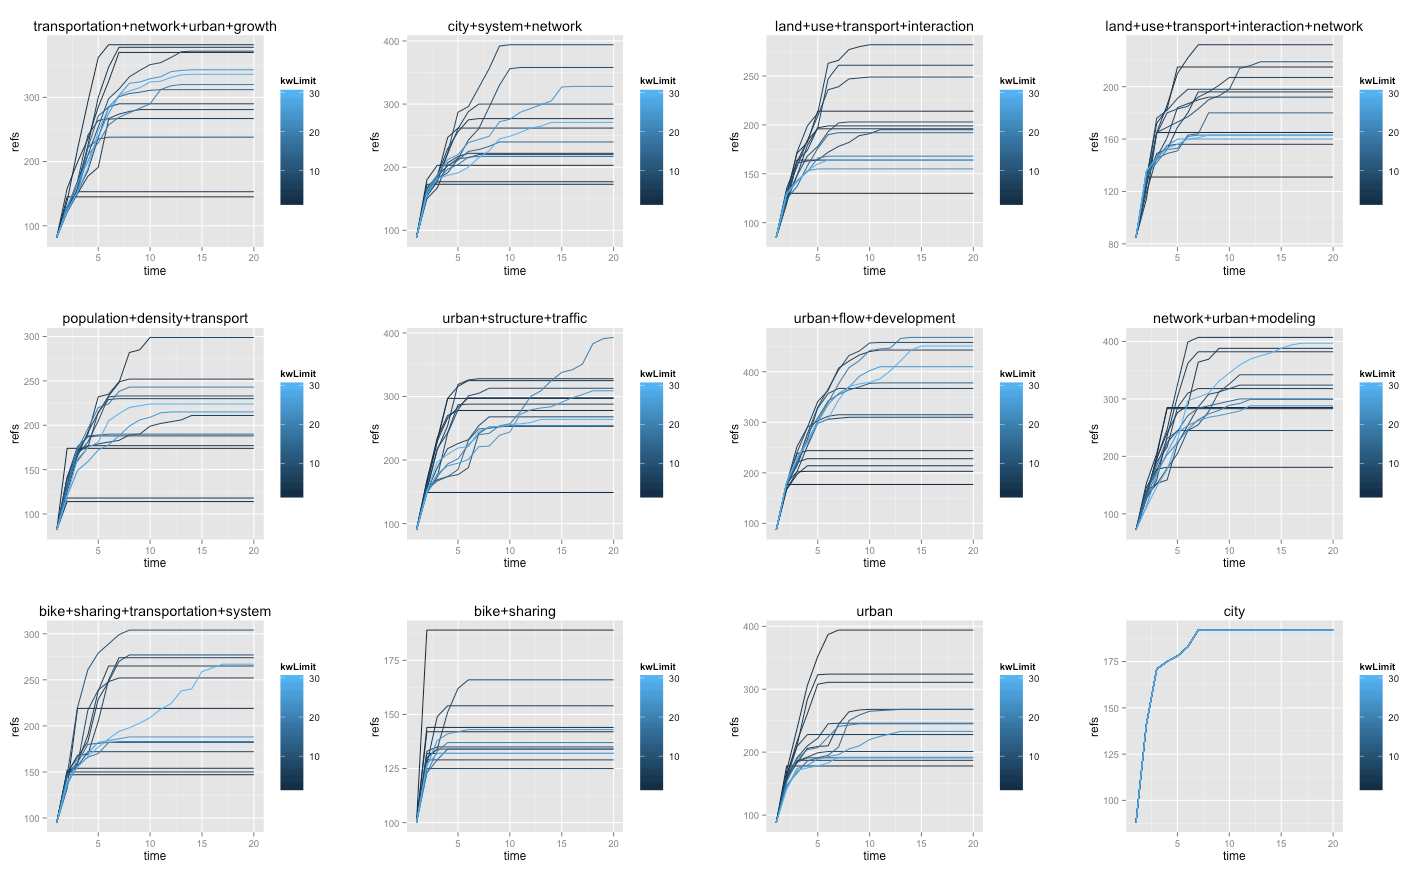
\includegraphics[width=\textwidth]{figures/resExpl_noException}
}
%%%%%%%%%%%%%%%%%%%%%%%%%%%%%%%%


%%%%%%%%%%%%%%%%%%%%%%%%%%%%%%%%
\jframe{Results : lexical consistence}{
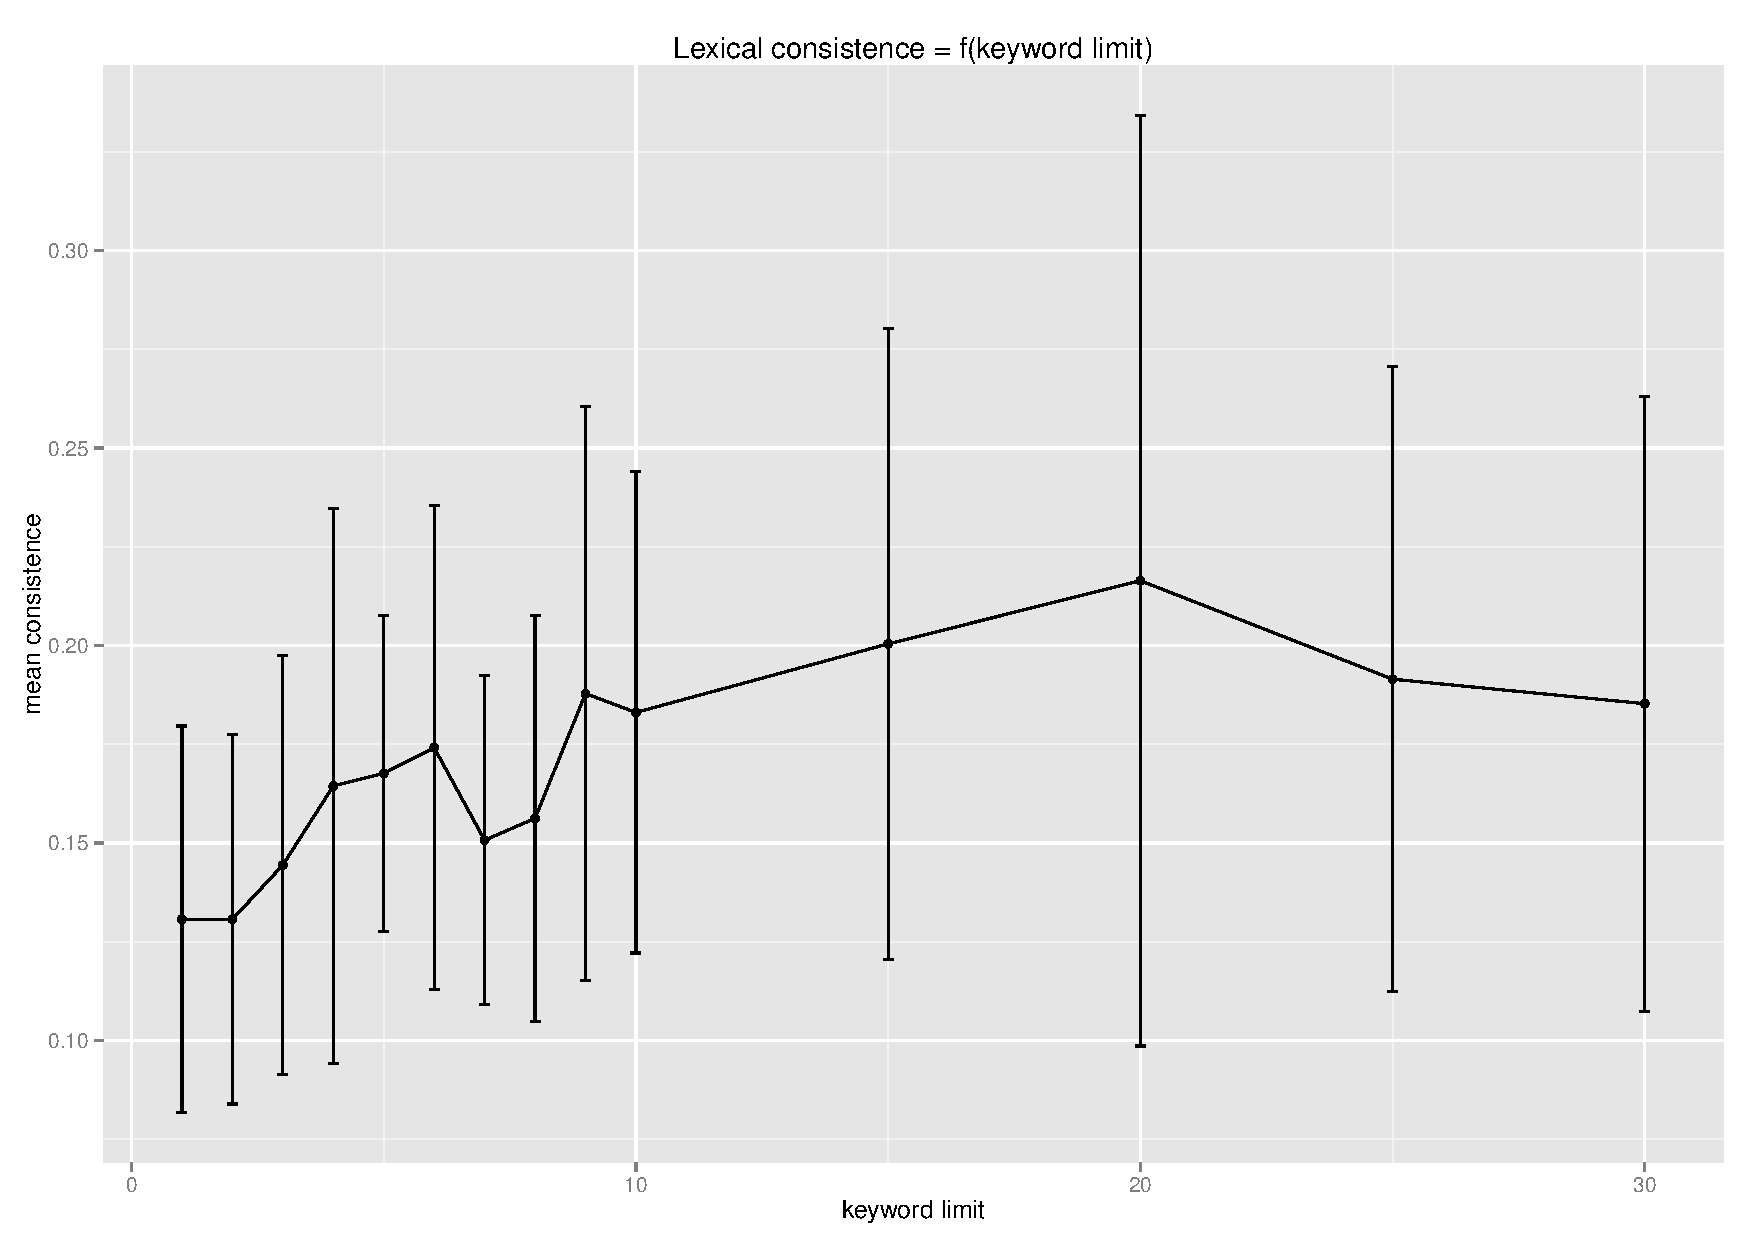
\includegraphics[width=\textwidth]{figures/lexicalConsistence_MeanSd}
}
%%%%%%%%%%%%%%%%%%%%%%%%%%%%%%%%





%%%%%%%%%%%%%%%%%%%%%%%%%%%%%%%%
\subsection{Reproducibility : models of network morphogenesis}

%%%%%%%%%%%%%%%%%%%%%%%%%%%%%%%%
\jframe{On the need of model formalization for reproducibility}{
Model for Tijuana bordertown, integrated in NL Urban Suite \cite{de2007netlogo}\\
Unvolontary falsification of results.\\
\medskip
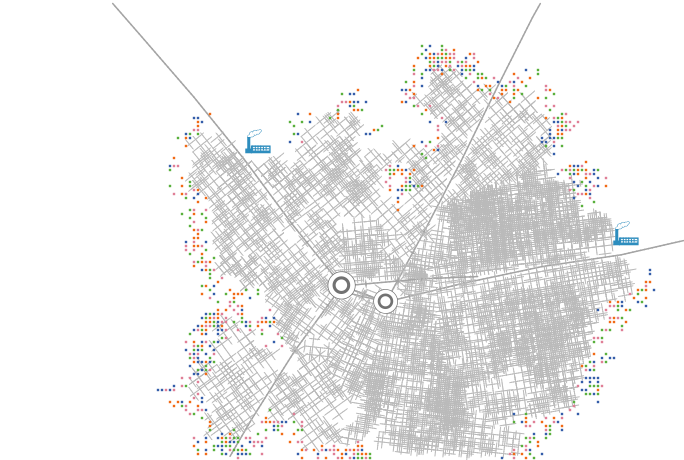
\includegraphics[width=0.28\textwidth]{figures/stdView}\hfill
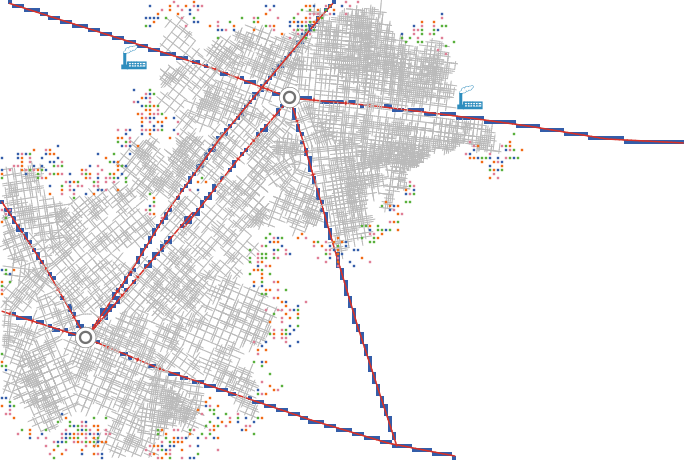
\includegraphics[width=0.28\textwidth]{figures/ViewRoads}
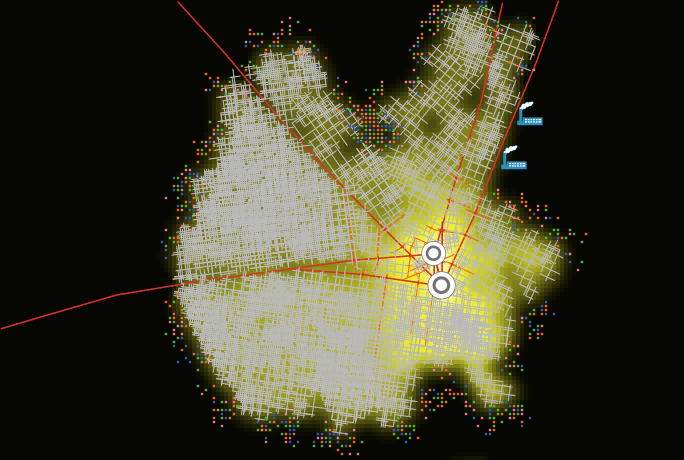
\includegraphics[width=0.28\textwidth]{figures/landValues_cityFinished}
}
%%%%%%%%%%%%%%%%%%%%%%%%%%%%%%%%

%%%%%%%%%%%%%%%%%%%%%%%%%%%%%%%%
\jframe{On the need of rigorous implementation}{
Geometrical street network growth model \cite{barthelemy2008modeling}\\
Non-reproducible results.\\
\medskip
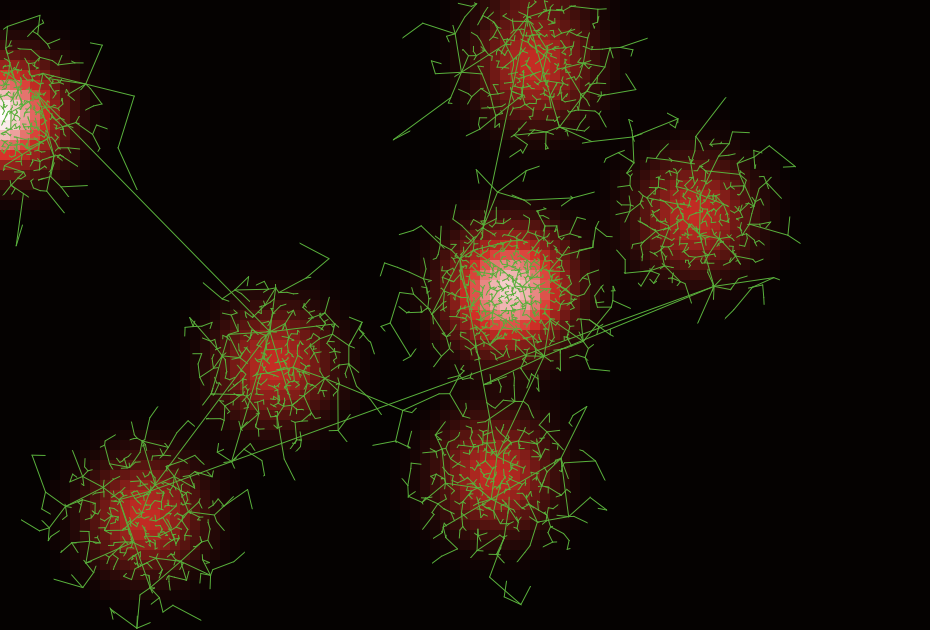
\includegraphics[width=0.48\textwidth]{figures/LocalDistanceMin_expProba_4000centers_withConnexNW}\hfill
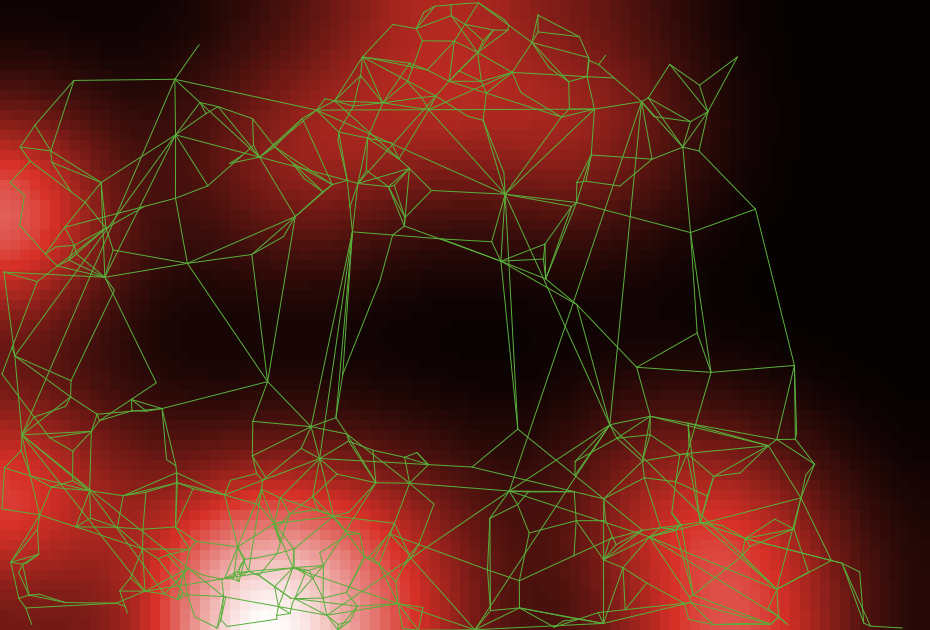
\includegraphics[width=0.48\textwidth]{figures/LocalDistanceMin_sharedNeighs_ExpMixt_11NewCenters}
}
%%%%%%%%%%%%%%%%%%%%%%%%%%%%%%%%




%%%%%%%%%%%%%%%%%%%%%%%%%%%%%%%%
\section{Next steps}

\begin{frame}
\frametitle{}

\vfill{}
 \begin{justify}
\textbf{Long Term Planning, 6 months}\\
State of the Art, Literature Review, Quantitative modelography, refined research question.
\end{justify}

\vfill{}
 \begin{justify}
\textbf{Short Term Planning, 1 month}\\
Finish systematic review (corpus synthesis, ``hand'' systematic review), implement and compare various models (ex. quantitative comparison of network growth models), test various paths (e.g. Florent's model on endogeneisation of transportation infrastructure evolution)
\end{justify}

\vfill{}
\vfill{}





\end{frame}






%%%%%%%%%%%%%%%%%%%%%%%%%%%%%%%%
\begin{frame}[allowframebreaks]
\frametitle{References}
\bibliographystyle{apalike}
\bibliography{/Users/Juste/Documents/ComplexSystems/CityNetwork/Biblio/Bibtex/CityNetwork,/Users/Juste/Documents/ComplexSystems/Biblio/Bibtex/global}
\end{frame}
%%%%%%%%%%%%%%%%%%%%%%%%%%%%%%%%


\end{document}